\documentclass{article}

\usepackage{tikz}
\usepackage{tikz-qtree}

\newcommand\leaf[3]{\makebox[5em][l]{#1}\texttt{#2\ldots#3\ldots}}

\newcommand\April     {\leaf{April     }{ 41 70 72 }{ 0100 0001 0111 0000 0111 0010 }} %      13.0
\newcommand\August    {\leaf{August    }{ 41 75 67 }{ 0100 0001 0111 0101 0110 0111 }} %      13.1  5.0
\newcommand\December  {\leaf{December  }{ 44 65 63 }{ 0100 0100 0110 0101 0110 0011 }} %       6.0  5.1  4.0
\newcommand\February  {\leaf{February  }{ 46 65 62 }{ 0100 0110 0110 0101 0110 0010 }} %       6.1
\newcommand\January   {\leaf{January   }{ 4a 61 6e }{ 0100 1010 0110 0001 0110 1110 }} %      11.0           3.0
\newcommand\July      {\leaf{July      }{ 4a 75 6c }{ 0100 1010 0111 0101 0110 1100 }} % 22.0 11.1  5.0
\newcommand\June      {\leaf{June      }{ 4a 75 6e }{ 0100 1010 0111 0101 0110 1110 }} % 22.1            4.1
\newcommand\March     {\leaf{March     }{ 4d 61 72 }{ 0100 1101 0110 0001 0111 0010 }} % 20.0
\newcommand\May       {\leaf{May       }{ 4d 61 79 }{ 0100 1101 0110 0001 0111 1001 }} % 20.1  6.0  5.1
\newcommand\November  {\leaf{November  }{ 4e 6f 76 }{ 0100 1110 0110 1111 0111 0110 }} %  7.0  6.1
\newcommand\October   {\leaf{October   }{ 4f 63 74 }{ 0100 1111 0110 0011 0111 0100 }} %  7.1
\newcommand\September {\leaf{September }{ 53 65 70 }{ 0101 0011 0110 0101 0111 0000 }} %                     3.1

\begin{document}

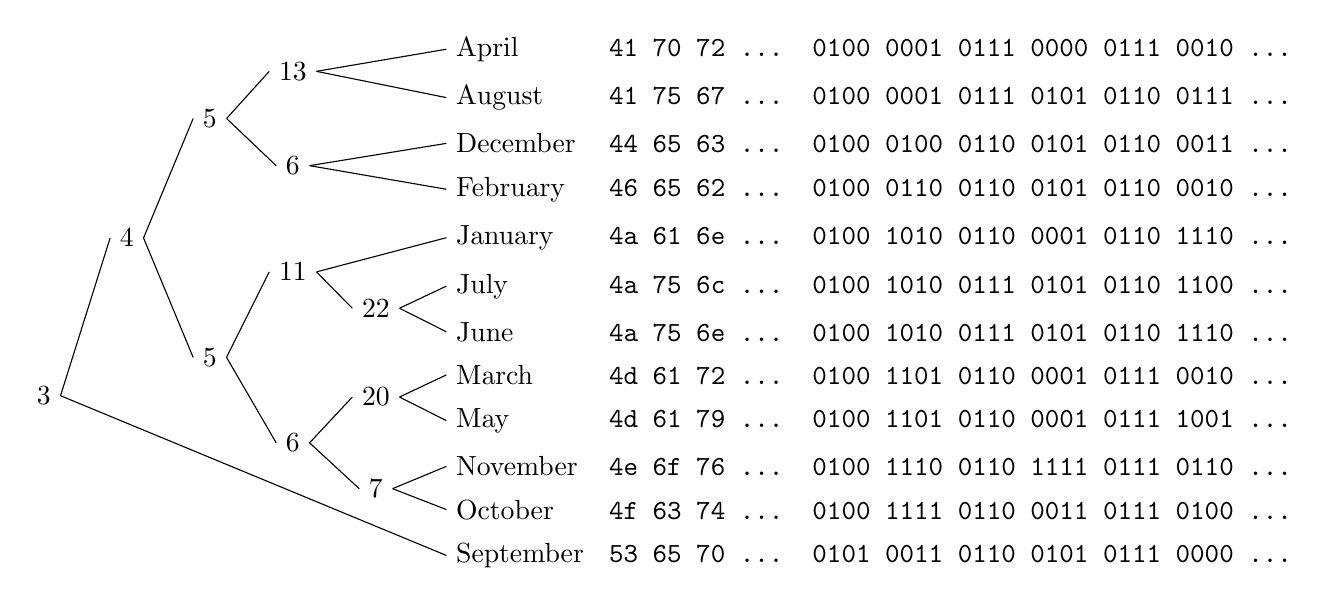
\begin{tikzpicture}

\tikzset{grow'=right,level distance=3em}
\tikzset{frontier/.style={distance from root=30em}}

\Tree [.3 [.4 [.5 [.13 {\April}
                       {\August} ]
                  [.6  {\December}
                       {\February} ] ]
              [.5 [.11 {\January}
                       [.22 {\July}
                            {\June} ] ]
                  [.6  [.20 {\March}
                            {\May} ]
                       [.7 {\November}
                           {\October} ] ] ] ]
          {\September} ]

\end{tikzpicture}

\end{document}
